% Created 2015-06-06 sam. 14:59
\documentclass[11pt,xcolor=dvipsnames,presentation]{beamer}
\usepackage[utf8]{inputenc}
\usepackage[T1]{fontenc}
\usepackage{fixltx2e}
\usepackage{graphicx}
\usepackage{longtable}
\usepackage{float}
\usepackage{wrapfig}
\usepackage{rotating}
\usepackage[normalem]{ulem}
\usepackage{amsmath}
\usepackage{textcomp}
\usepackage{marvosym}
\usepackage{wasysym}
\usepackage{amssymb}
\usepackage{hyperref}
\tolerance=1000
\usedescriptionitemofwidthas{bl}
\usepackage[T1]{fontenc}
\usepackage[utf8]{inputenc}
\usepackage[american, english]{babel}
\usepackage{ifthen,figlatex,amsmath,amstext,gensymb,amssymb}
\usepackage{boxedminipage,xspace,multicol}
%%%%%%%%% Begin of Beamer Layout %%%%%%%%%%%%%
\ProcessOptionsBeamer
\usecolortheme{whale}
\usecolortheme[named=BrickRed]{structure}
\useinnertheme{rounded}
\useoutertheme{infolines}
\setbeamertemplate{footline}[frame number]
\setbeamertemplate{headline}[default]
\setbeamertemplate{navigation symbols}{}
\defbeamertemplate*{headline}{info theme}{}
\defbeamertemplate*{footline}{info theme}{\leavevmode%
\hbox{%
\begin{beamercolorbox}[wd=.2\paperwidth,ht=2.25ex,dp=1ex,center]{author in head/foot}%
\usebeamerfont{author in head/foot}\insertshortauthor
\end{beamercolorbox}%
\begin{beamercolorbox}[wd=.71\paperwidth,ht=2.25ex,dp=1ex,center]{title in head/foot}%
\usebeamerfont{title in head/foot}\insertsectionhead
\end{beamercolorbox}%
\begin{beamercolorbox}[wd=.09\paperwidth,ht=2.25ex,dp=1ex,right]{section in head/foot}%
\usebeamerfont{section in head/foot}\insertframenumber{}~/~\inserttotalframenumber\hspace*{2ex}
\end{beamercolorbox}
}\vskip0pt}
\setbeamertemplate{footline}[info theme]
%%%%%%%%% End of Beamer Layout %%%%%%%%%%%%%
\usepackage{verbments}
\usepackage{xcolor}
\usepackage{color}
\usepackage{url} \urlstyle{sf}
\let\alert=\structure % to make sure the org * * works of tools
\usetheme{default}
\author{Steven QUINITO MASNADA}
\date{Grenoble, 8 Juin 2015}
\title{\textbf{TER} \\ Simulation d'application dynamiques pour plateformes de calculs hautes performances \bigskip\\ \large Équipe MESCAL}
\hypersetup{
  pdfkeywords={},
  pdfsubject={},
  pdfcreator={Emacs 24.5.1 (Org mode 8.2.10)}}
\begin{document}

\maketitle


\section{Présentation générale}
\label{sec-1}
\begin{frame}[label=sec-1-1]{Présentation générale}
TER dans l'équipe MESCAL, encadré par Arnaud LEGRAND et Luka STANISIC 
\end{frame}
\section{Contexte et problèmatique}
\label{sec-2}
\begin{frame}[label=sec-2-1]{Architecture et standard HPC}
\begin{figure}[tbh]
\centering
\vspace{-1.5mm}
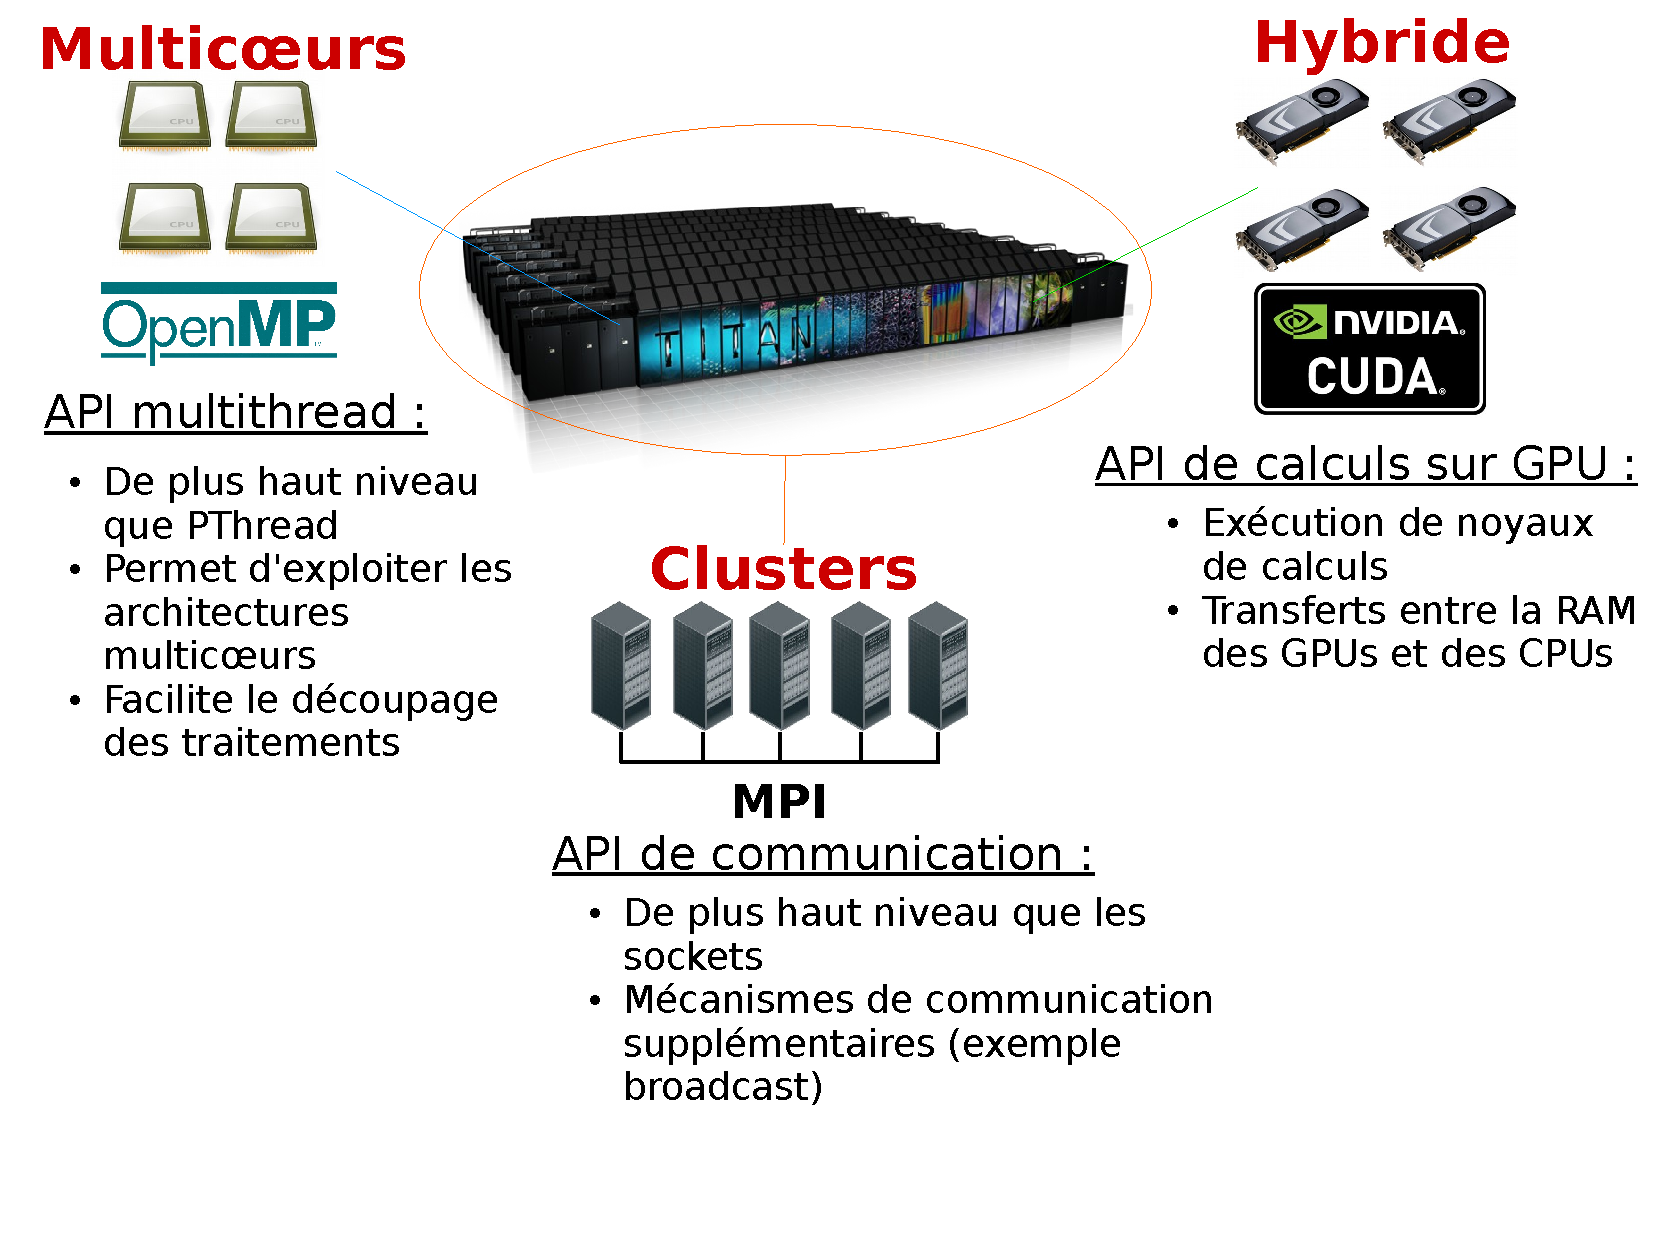
\includegraphics[width=\linewidth]{./Slides/Archi.pdf}
\end{figure}
\end{frame}

\begin{frame}[label=sec-2-2]{Limites des approches classiques}
\begin{itemize}
\item Utiliser \alert{plusieurs paradigmes} $\leadsto$ \alert{programmation complexe}
\item Exemple pour exploiter efficacement un GPU sur \alert{un seul noeud}:
\begin{itemize}
\item \alert{transférer données} du CPU au GPU,
\item \alert{lancer le calcul} sur le GPU
\item \alert{gérer synchronisation} pendant attente résultat
\item \alert{occuper} CPU
\item \alert{récupérer} résultat.
\end{itemize}
\item Et avec \alert{plusieurs noeuds}?
\item \alert{Statique}, système réglé comme un horloge $\leadsto$ pas portable.
\item Solution: \alert{Dynamique} mais presque \alert{impossible avec APIs classiques}.
\end{itemize}
\end{frame}
\begin{frame}[label=sec-2-3]{Nouvelle approche: Paradigme de tâches}
\begin{columns}
  \begin{column}{.55\linewidth}
\begin{itemize}
\item Nouvelle abstraction: les tâches
\begin{itemize}
\item \alert{Plus besoin de se soucier de la ressource} sur laquelle le
traitement est effectué.
\item Exprimer calcul en \alert{graphe de tâches} $\leadsto$ système dynamique
plus simple.
\end{itemize}
\end{itemize}

  \end{column}
  \begin{column}{.35\linewidth}
    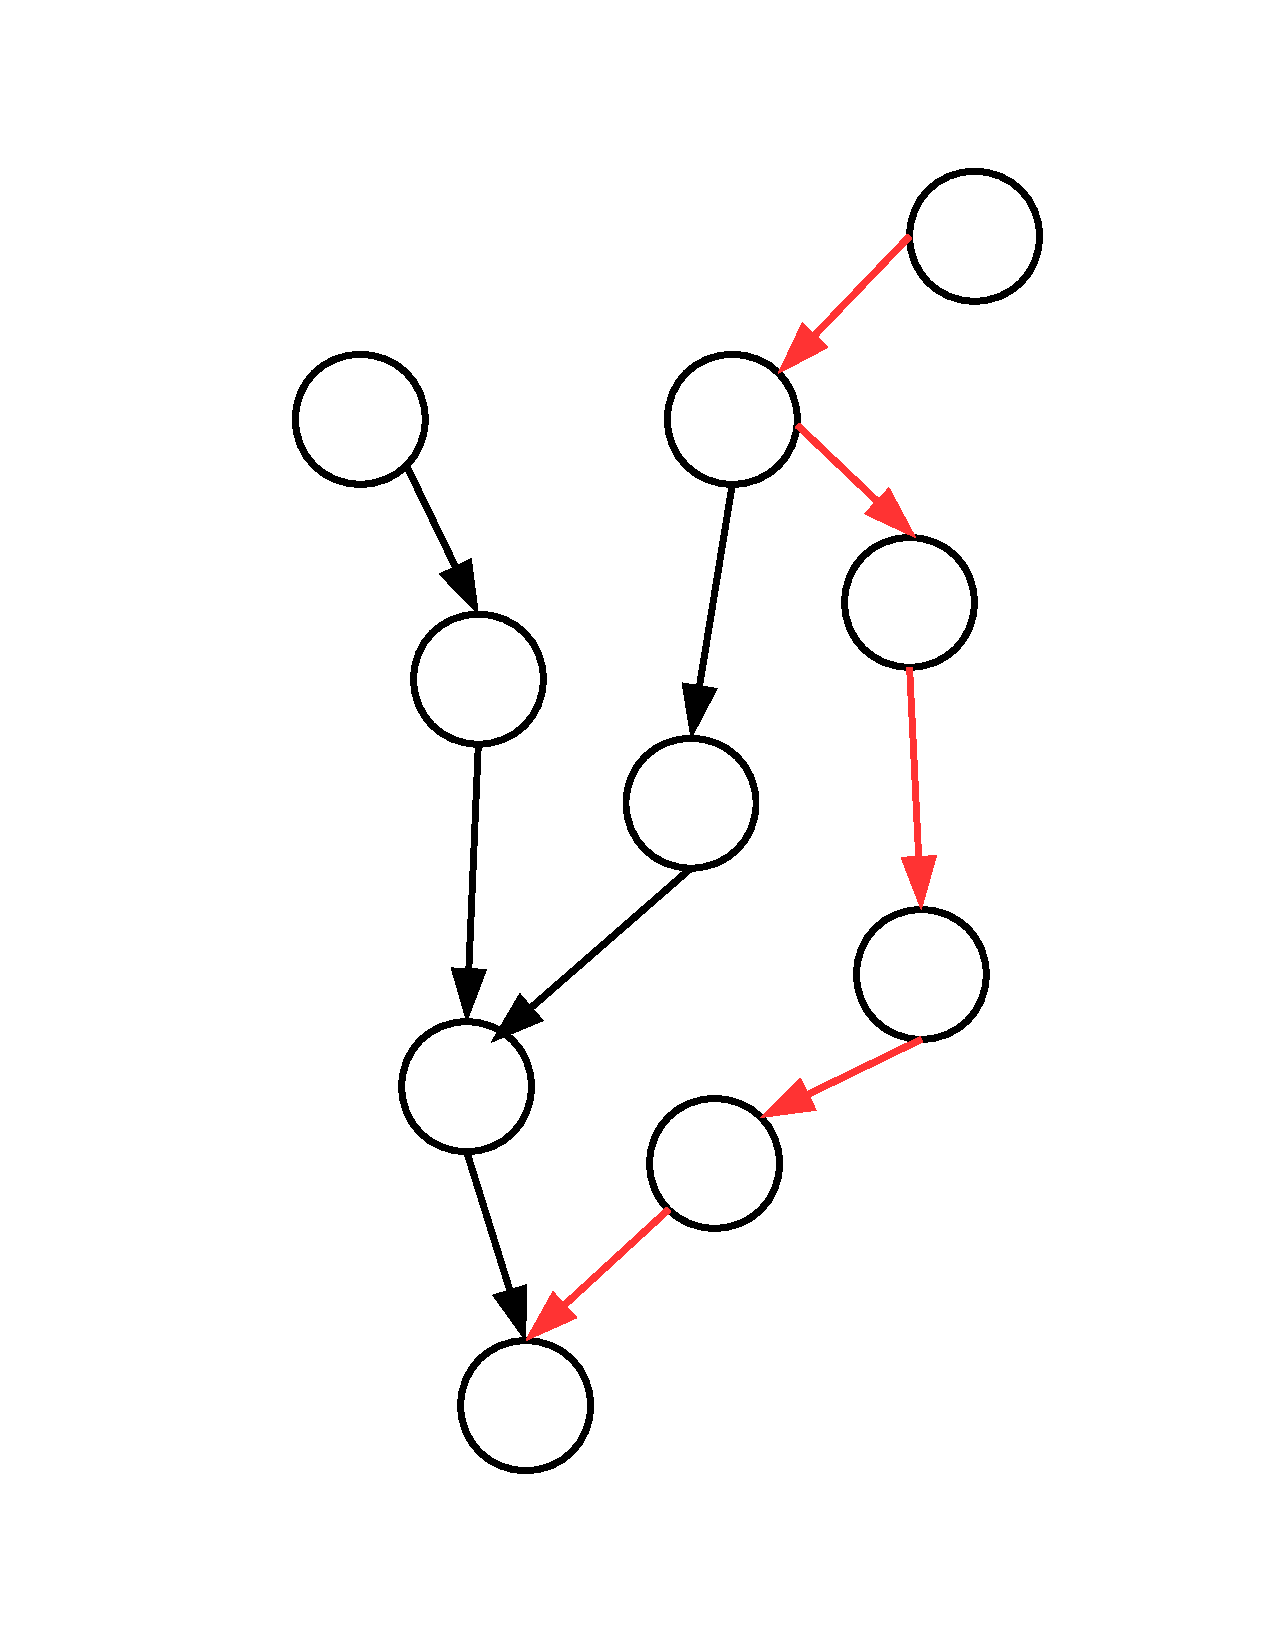
\includegraphics[width=.45\linewidth]{img/task_graph.jpg}%
  \end{column}
\end{columns}

\begin{itemize}
\item Librairie StarPU:
\begin{itemize}
\item Système \alert{runtime}
\item basé sur le paradigme de tâches $\leadsto$ graphe de dépendances.
\item Ordonnancemment \alert{dynamique et opportuniste}.
\end{itemize}
\item Problèmatique : Performances difficiles à évaluer
\begin{itemize}
\item Configuration \alert{runtinme}, heuristique, politique ordonnancement.
\item Configuration \alert{application}, découpage des tâches.
\end{itemize}
\end{itemize}
\end{frame}
\section{État de l'art}
\label{sec-3}
\begin{frame}[label=sec-3-1]{Test sur systèmes réels}
\begin{itemize}
\item Exécution réelle sur la plateforme cible $\leadsto$ \alert{coûteux}
\item Exéuction \alert{non déterministe} nécessite de réaliser beaucoup
d'expériences $\leadsto$ extrapolations difficiles.
\end{itemize}
\end{frame}
\begin{frame}[label=sec-3-2]{Simulation}
\begin{block}{Généralités}
\begin{itemize}
\item Utilisation de \alert{modèles} pour \alert{prédire} comportements.
\item Permet s'affranchir de la plateforme $\leadsto$ peu coûteux.
\item Contrôle paramètres $\leadsto$ \alert{systèmes déterministes}.
\item Extrapolation simplifiée.
\item Exécution plus courte.
\end{itemize}
\end{block}

\begin{block}{Simulation par rejeu de trace}
Exécution post-mortem: pas adapté ici car \alert{flot de contrôle non
déterministe}.
\end{block}
\begin{block}{Hybride simulation / émulation}
\begin{itemize}
\item Simuler plateforme et OS.
\item Emuler de l'application.
\end{itemize}
\end{block}
\begin{block}{Choix}
\end{block}
\end{frame}
\section{Analyse du problème}
\label{sec-4}
\begin{frame}[label=sec-4-1]{SimGrid}
\end{frame}
\begin{frame}[label=sec-4-2]{StarPU MSG}
\end{frame}
\begin{frame}[label=sec-4-3]{StarPU SMPI}
\end{frame}

\section{Méthodologie}
\label{sec-5}
\section{Contribution}
\label{sec-6}
\section{Validation}
\label{sec-7}
\section{Conclusion}
\label{sec-8}


\section{General Presentation}
\label{sec-9}
\begin{frame}[label=sec-9-1]{Project-Team Composition}
\begin{itemize}
\item \alert{\textit{Natural} evolution} of the MESCAL team.\vspace{-1em}
\end{itemize}

\null\hspace{-1em}\hbox{\scalebox{.82}{
\begin{tabular}{llll}
  Name & Affiliation & Provenance & Expertise\\
  \hline
  V. Danjean & MdC UJF & MOAIS & HPC, Tracing, Experimental Methodology\\
  N. Gast & CR2 Inria & MESCAL & Optimization, Stochastic Modeling\\
  B. Gaujal & DR1 Inria & MESCAL & Modeling, Optimization, Game Theory\\
  G. Huard & MdC UJF & MOAIS & HPC, Tracing, Visualization\\
  A. Legrand & CR1 CNRS & MESCAL & HPC, Simulation, Visualization, Optimization\\
  F. Perronnin & MdC UJF & MESCAL & Simulation, Stochastic and fluid models\\
  P. Mertikopoulos & CR2 CNRS & MESCAL & Optimization, Game/Information Theory\\
  J.M. Vincent & MdC UJF & MESCAL & HPC, Modeling, Simulation, Visualization\\
\end{tabular}
}\hspace{-2em}}

\begin{itemize}
\item \alert{Inria field / theme:} 
\begin{itemize}
\item Network, Systems and Services
\item Distributed Computing / Distributed and High Performance Computing
\end{itemize}
\item \alert{Keywords}: HPC/large distributed systems, performance analysis,
distributed and stochastic optimization, \ldots{}
\end{itemize}
\end{frame}

\begin{frame}[label=sec-9-2]{Context and Objectives}
\begin{itemize}
\item \alert{Large distributed infrastructures}
\vspace{-1em}\begin{multicols}{2}
\begin{itemize}
\item \textbf{HPC/cloud/...}
\item Wireless networks
\item Smart grids
\item Transportation systems
\end{itemize}
\end{multicols}
\hbox{\hspace{-.7cm}%
  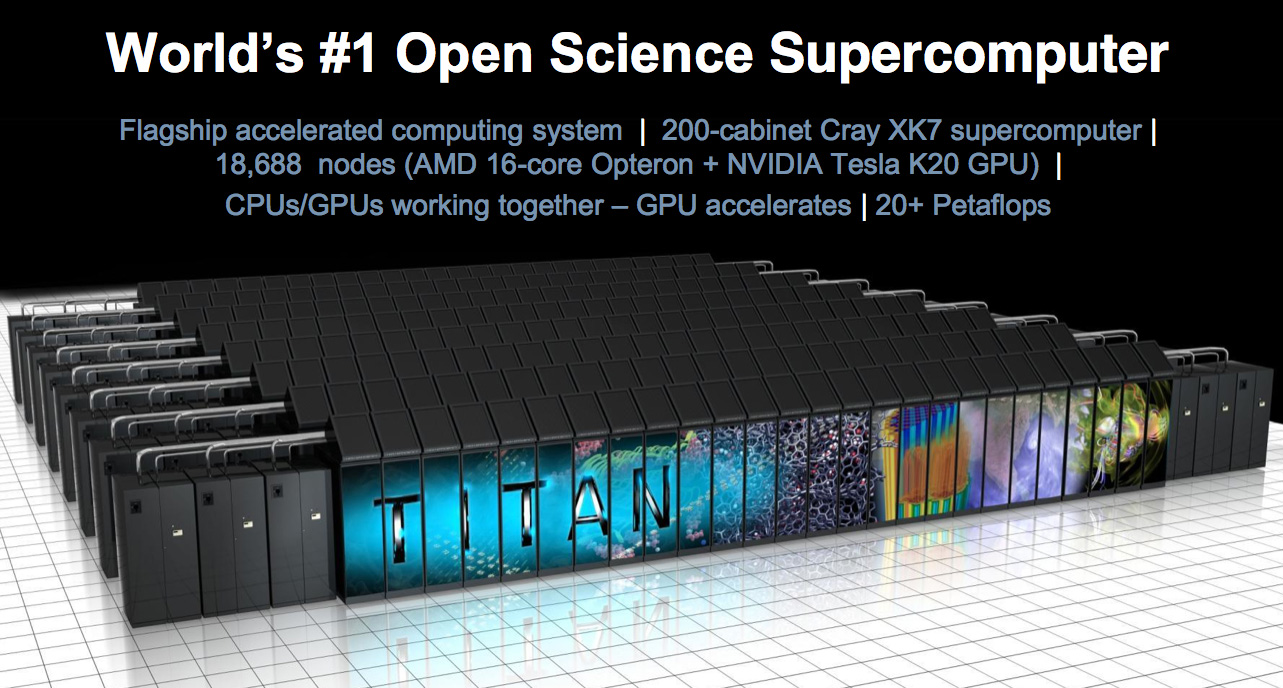
\includegraphics[height=2.15cm]{img/plat_titan.jpg}
  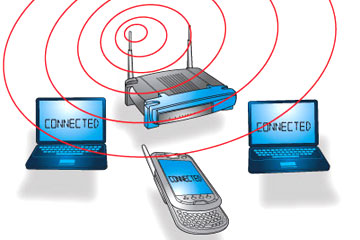
\includegraphics[height=2.15cm]{img/plat_wireless.jpg}
  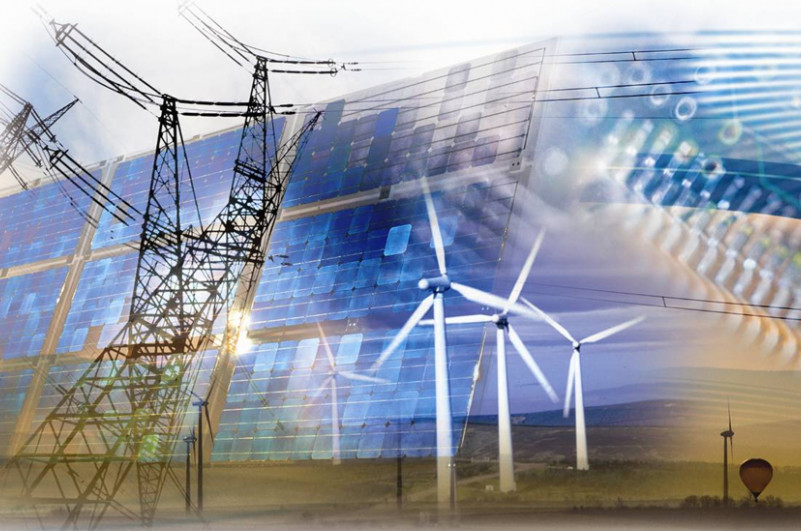
\includegraphics[height=2.15cm]{img/plat_smartgrid.jpg}
  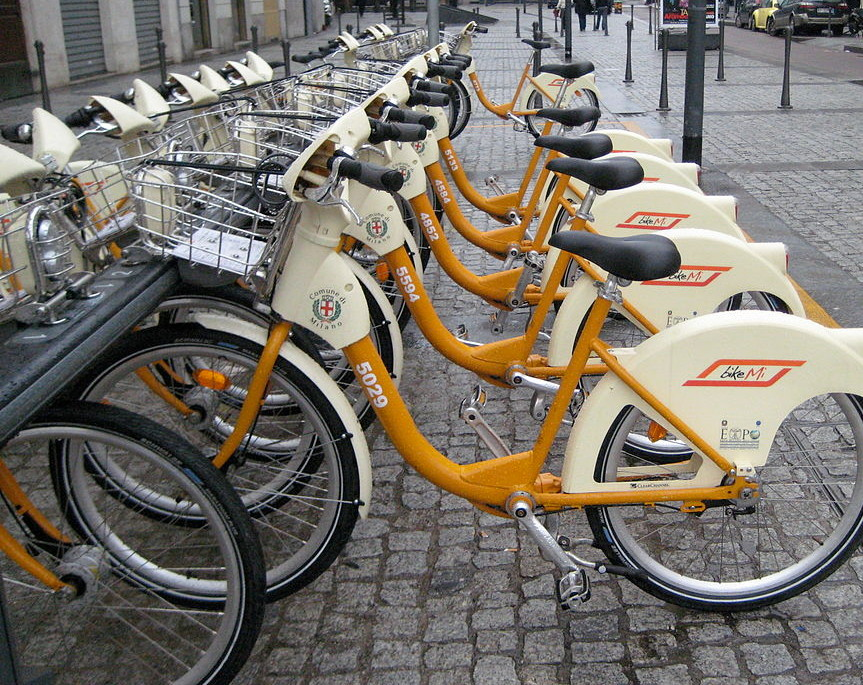
\includegraphics[height=2.15cm]{img/plat_bikesharing.jpg}%
}
\item \alert{Common questions} scalability, resilience, adaptability, capacity
planning, energy consumption, \dots{}
\item \alert{Common characteristics} ever growing size, distributed,
heterogeneous, user-centric $\leadsto$ \alert{stochastic nature}
\end{itemize}
\begin{itemize}
\item This requires \alert{involved tools and new techniques} that will be useful
to the D\&HPC community
\end{itemize}
\end{frame}

\begin{frame}[label=sec-9-3]{Scientific Foundations: POLARIS in a Nutshell}
\begin{quote}
\alert{Contribute to the understanding} (from the \alert{observation}, \alert{modeling and
analysis} to the \alert{optimization} through adapted algorithms) \alert{of
performances of very large scale distributed computing systems} by
applying original ideas from \alert{other research fields and application
domains}.
\end{quote}
{\bf
POLARIS = \alert{Team} of people with the right spectrum of \alert{skills}
}
\begin{description}
\item[{Experiment design}] measuring/monitoring/tracing tools, experimental methodology
(design, control, reproducibility)
\item[{Modeling and Simulation}] discrete event simulation, emulation,
Markov chains, perfect sampling, Monte Carlo methods, \ldots{}
\item[{Visualization and Statistical Analysis}] workload characterization (failures, parallel systems),
visualization and analysis of parallel applications
\item[{Optimization}] stochastic approximations, mean field limits, game
theory, mean field games, primal dual optimization,
learning, information theory
\end{description}
\end{frame}

\begin{frame}[label=sec-9-4]{Research Methodology}
A continuum of 5 research areas
\begin{columns}
  \begin{column}{.05\linewidth}
   \vspace{.8em}
   
\includegraphics[height=4.6cm]{img/arrow.pdf}
  \end{column}
  \begin{column}{.9\linewidth}
\begin{itemize}
\item \textbf<2>{\alert{Measurement}}
design of experiments, observation
overhead control, reproducible research
\item \alert{Visualization} performance qualification and debugging, multi-scale
visualization, trace comparison
\item \textbf<2>{\alert{Simulation}}
faithful simulation of HPC systems, sensibility/robustness,
trajectory coupling
\item \alert{Fluid Modeling} local interactions, transient analysis
\item \alert{Optimization} learning algorithms in continuous nonlinear games,
online and distributed optimization
\end{itemize}
  \end{column}
\end{columns}
\end{frame}
\section{Research Direction}
\label{sec-10}
\begin{frame}[label=sec-10-1]{\textbf{Measurement:} Reproducible Experimental Methodology}
Real experiments are \alert{costly}, \alert{difficult} to \alert{control} and to \alert{reproduce}
\begin{itemize}
\item \small Cannot be studied anymore like artificial systems. Need to
\alert{inspire from other experimental fields}
\end{itemize}

\textbf{Research directions}:
\begin{itemize}
\item \alert{Design of experiments}: involved statistical technique widely used in
all fields where experiments are expensive but CS
\begin{itemize}
\item \alert{Bridge} this \alert{gap} and \alert{favor its adoption} in the D\&HPC theme
\end{itemize}
\item \alert{Monitoring and tracing}: need for multi-scale
(application/space/time) observation where intrusiveness is
controlled
\begin{itemize}
\item Evaluate the \alert{observation/analysis quality trade-off}
\end{itemize}
\item \alert{Open science and reproducibility}: complexity and rapid technological
evolution = excuse for not taking care of results reproducibility
\begin{itemize}
\item Monitor/document the whole process (design, execution, data
gathering, filtering, analysis)
\item Investigate/design \alert{pragmatic workflows} to alleviate this flaw
\end{itemize}
\end{itemize}
\end{frame}
\begin{frame}[label=sec-10-2]{\textbf{Visualization:} "Performance Driver" Identification}
Traditional approach: display \alert{everything}\\
\only<2>{$\leadsto$ harmful \alert{biases} (\emph{more information than what fits on your screen})}
  \begin{overlayarea}{\linewidth}{3.7cm}
    \only<1>{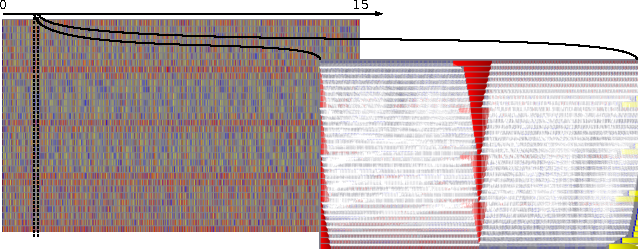
\includegraphics[width=\linewidth]{img/trace_zoom.pdf}}%
    \pause%
    \vspace{-.5em}
    \begin{center}
      \begin{tabular}{cc}
        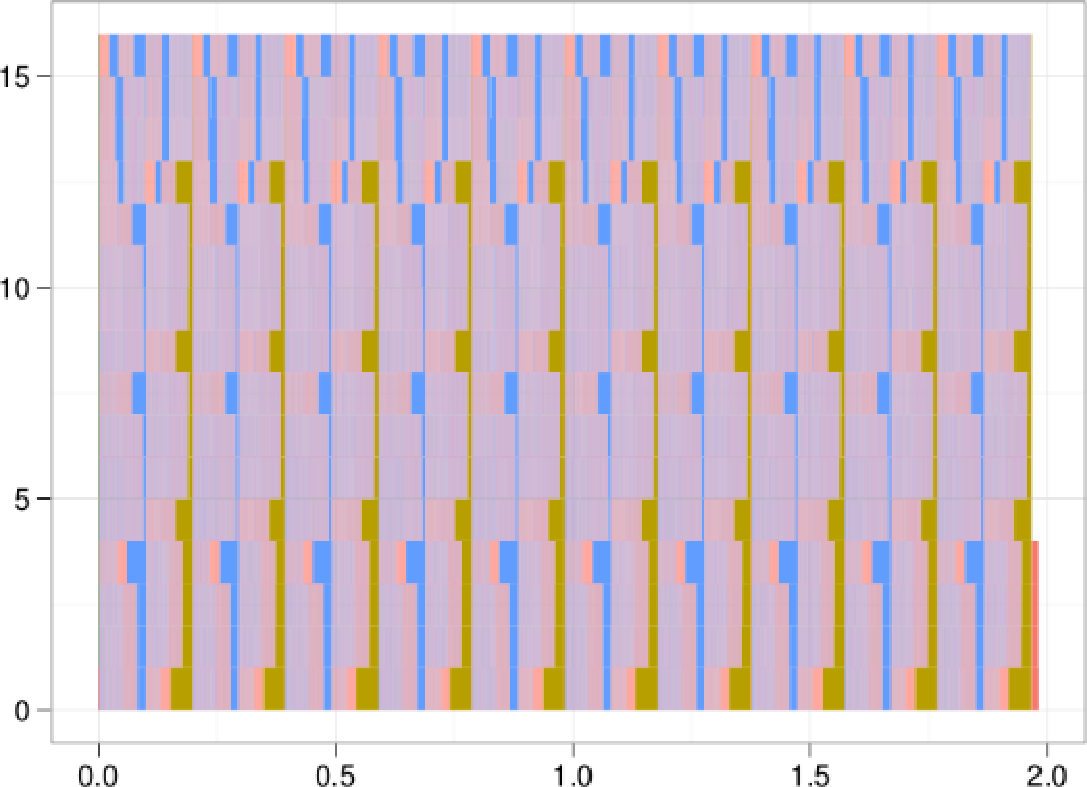
\includegraphics[width=.3\textwidth]{img/r_gantt_evince.pdf} & 
        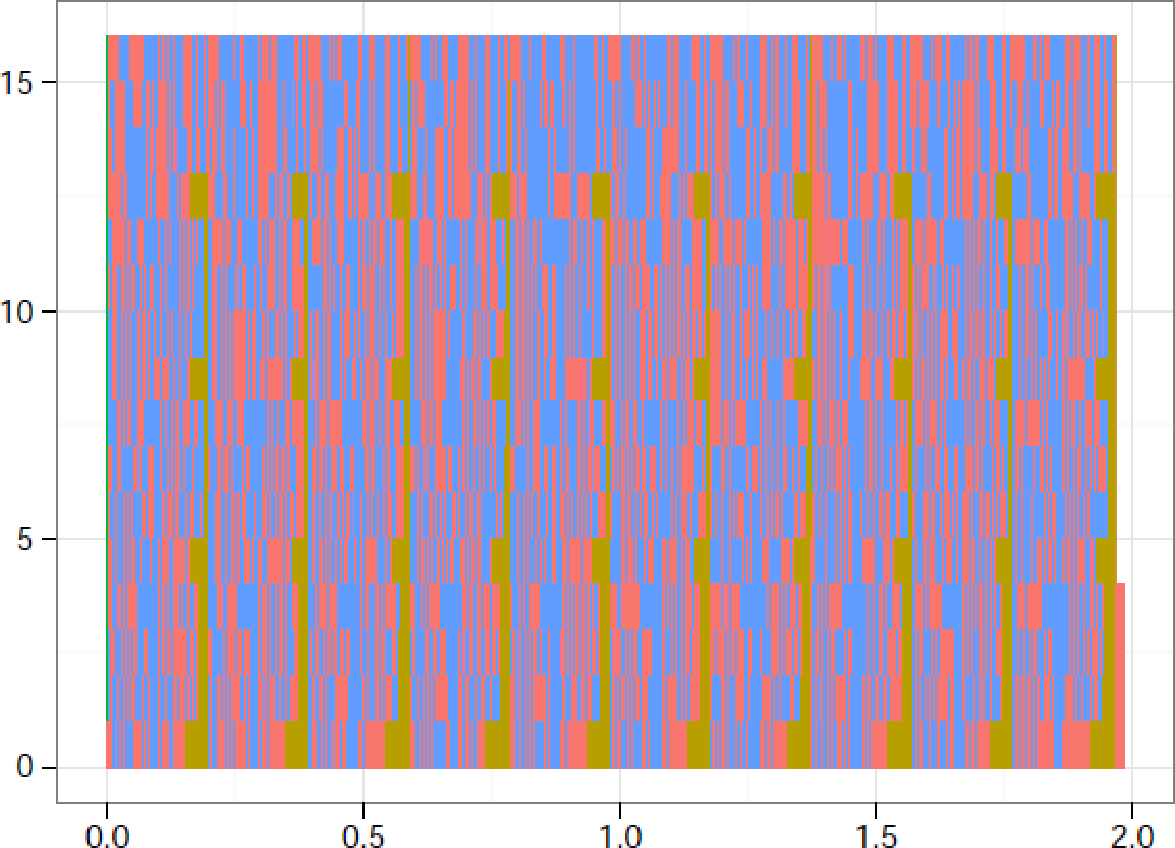
\includegraphics[width=.3\textwidth]{img/r_gantt_acroread.pdf} \\
        Evince & Acroread
      \end{tabular}
    \end{center}
    \vspace{-1em}
   \hbox{$\leadsto$ \emph{overenthusiastic} use of \emph{clustering}, pattern \emph{mining}, \emph{sequence alignment}}
  \end{overlayarea}
\textbf{Research Directions}:
\begin{itemize}
\item Performance \alert{qualification} and \alert{debugging}
\begin{itemize}
\item Colleagues from D\&HPC theme in deep need of new approaches/tools
\end{itemize}
\item \alert{Multi-scale} analysis (space/time/application) resilient to \alert{noise}
\begin{itemize}
\item \alert{Entropy-based Aggregation} applied to embedded/HPC systems
\end{itemize}
\item Trace \alert{comparison}\smallskip
\end{itemize}
\end{frame}
\begin{frame}[label=sec-10-3]{\textbf{Simulation:} Very Large Stochastic Systems}
\begin{itemize}
\item Simulation circumvents some of the previous experimental issues
\begin{itemize}
\item cost/screening, extrapolation, capacity planning, \ldots{}
\end{itemize}
\item Traditional approach: simplistic models to study large-scale
systems, developed by D\&HPC experts who know little about simulation
\begin{itemize}
\item \alert{Short-lived} tools with \alert{no intent of predicting} anything. At best
grossly indicates trend but no more expectation
\end{itemize}
\end{itemize}
\textbf{Research directions}:
\begin{itemize}
\item Accurately \alert{reproduce the dynamic of real systems}
\begin{itemize}
\item \alert{SimGrid}: Versatile simulation of large-scale distributed systems \\
    \alert{coarse-grain fluid models}, mix \alert{emulation/simulation}, \alert{invalidation}
\item Used is RUNTIME/HIEPACS, ASCOLA, KERDATA, AVALON, \dots{}
\end{itemize}
\item Provide \alert{sensibility} analysis and \alert{robustness} indicators
\item Trajectory \alert{coupling} for discrete event simulations
\begin{itemize}
\item \alert{PSI$^2$}: Perfect sampling for Markovian systems
\end{itemize}
\end{itemize}
\uncover<2>{
\begin{overlayarea}{\linewidth}{0cm}
  \vspace{-7.5cm}
  \begin{center}
    \begin{minipage}{\linewidth}
      \begin{exampleblock}{Simulation of Cholesky/StarPU on a hybrid platform}
        \begin{center}
          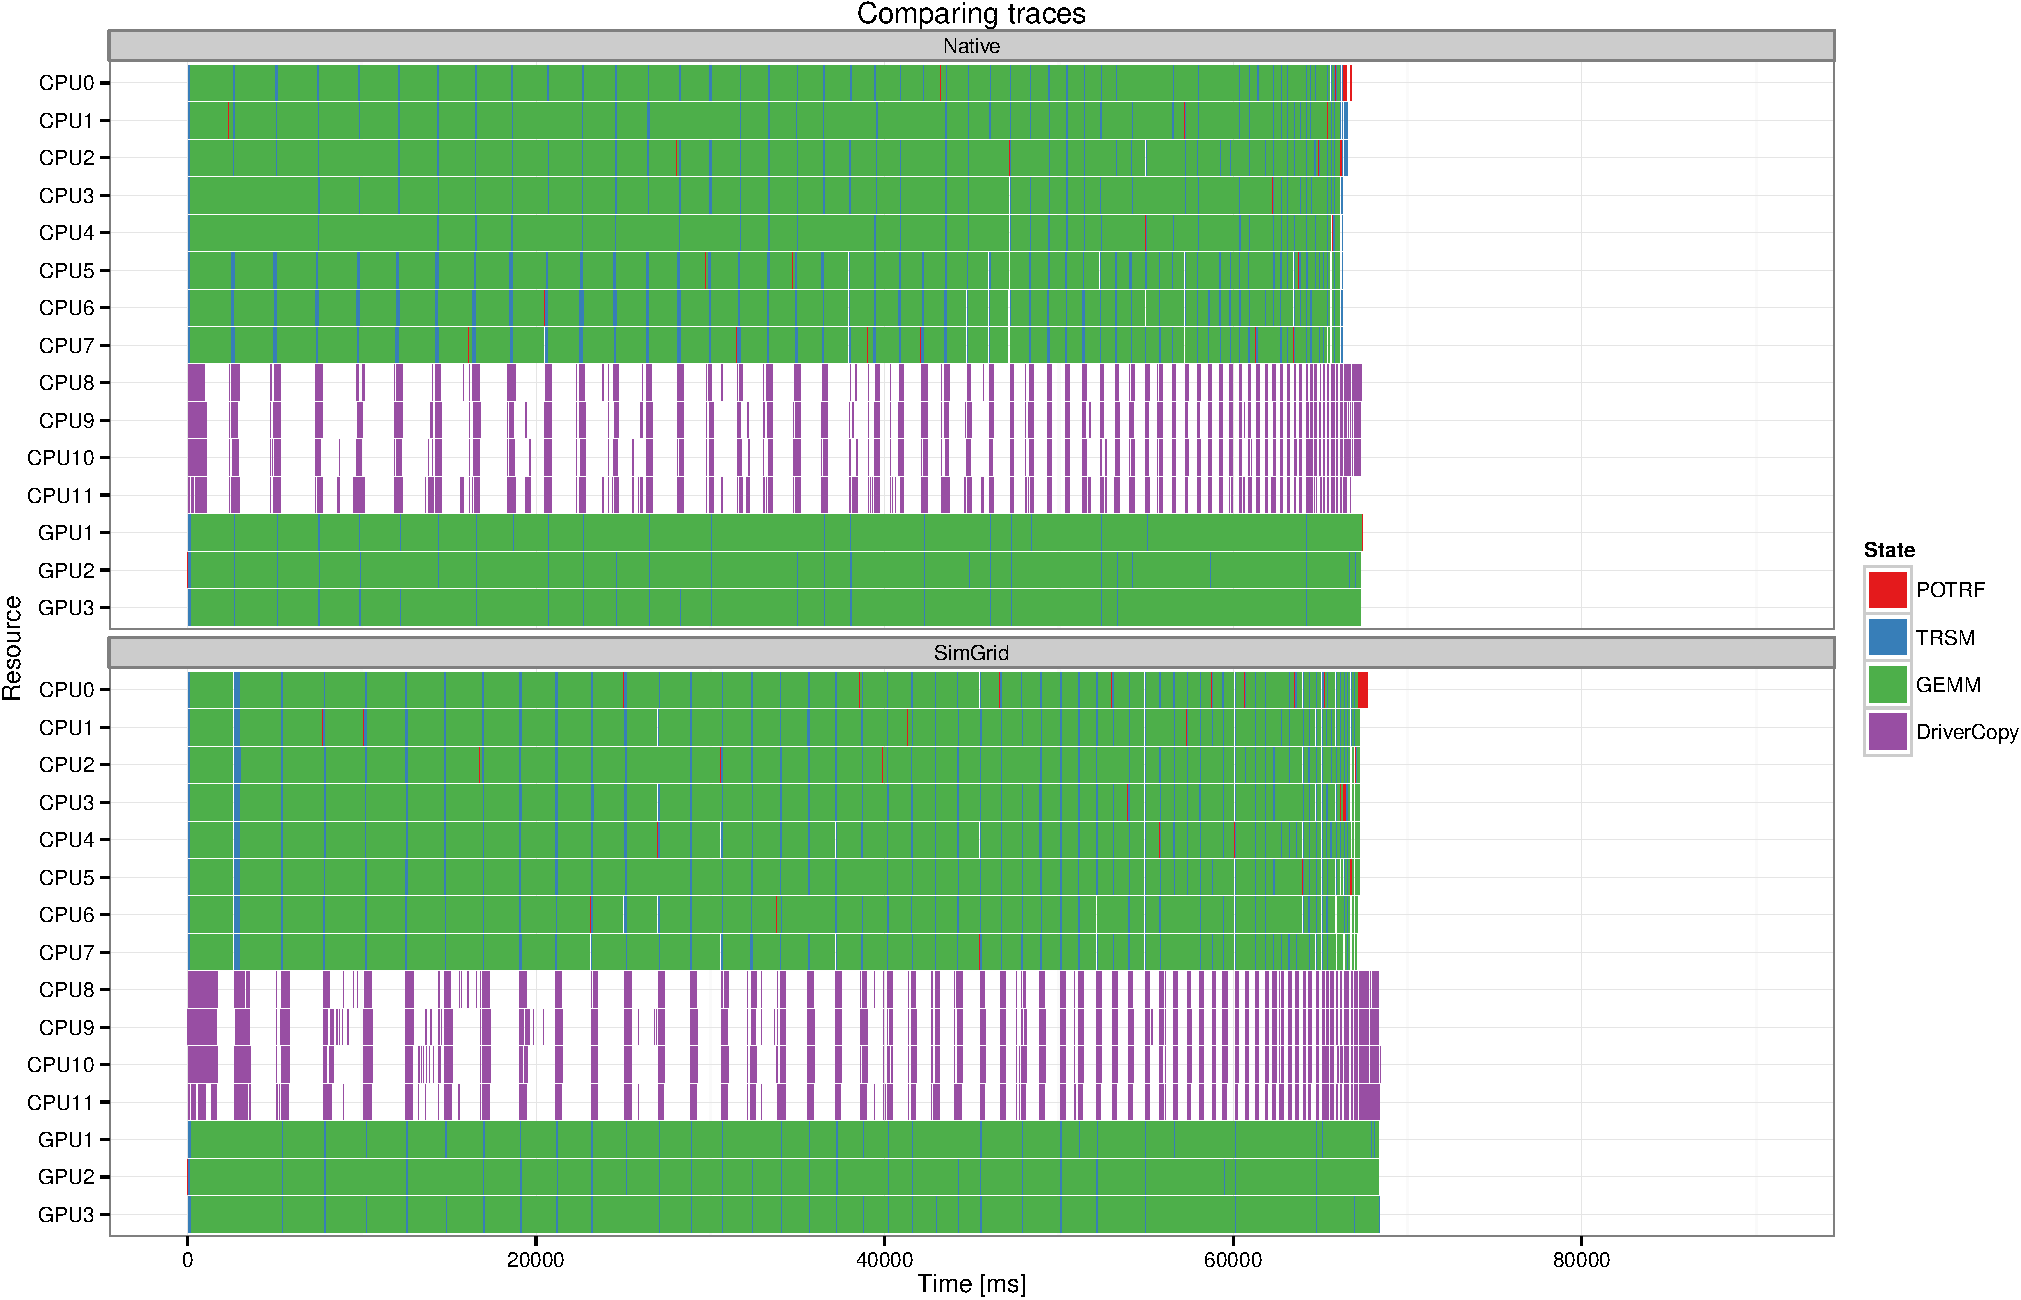
\includegraphics[width=.8\linewidth]{img/comparing_hybrid_mkl-crop.pdf}
        \end{center}
      \end{exampleblock}
    \end{minipage}
  \end{center}
\end{overlayarea}}\medskip
\end{frame}

\begin{frame}[label=sec-10-4]{\textbf{Analysis:} Local Interactions and Transient Analysis}
Analysis of \alert{stochastic} systems is particularly difficult
but \alert{mean-field} approximation is suited to \alert{large systems}
\begin{itemize}
\item \alert{Key hypothesis}: the dynamic solely depends
on the entity state (not on their identity nor on their spatial
location) and state space does not scale
\end{itemize}

\textbf{Research directions}:
\begin{itemize}
\item \alert{Locality is essential}: possible approaches
\begin{itemize}
\item pair approximation from statistical physics
\item fixed interaction graphs and a multi-scale approach
\item \emph{never used for distributed computing systems and high potential}
\end{itemize}

\item \alert{Transient behavior}:
\begin{itemize}
\item Finite horizon: OK (discrete system is uniformly close to
its continuous limit)
\item Infinite time horizon when the continuous limit is globally
stable: OK
\item Trajectory dependent stopping time: ???
\item \emph{Could be used to analyze the complexity of distributed algorithms}
\end{itemize}
\end{itemize}
\end{frame}
\begin{frame}[label=sec-10-5]{Optimization}
\frametitle{\textbf{Optimization:} \scalebox{.92}{\hbox{Game Theory, On-line Distributed~Optimization\hspace{-1em}}}}
\begin{block}{Modeling interactions through \alert{game theory}}
\vspace{-.5em}
Nash equilibrium often inefficient but \alert{efficient equilibrium} can be
\alert{learned} \small\vspace{-.6em}
\begin{itemize}
\item Finite set of strategies = OK. \textbf{In}finite set = ???\vspace{-.6em}
\begin{itemize}
\item Examples: routing packet flows, power control in wireless
networks, \dots{}
\item Discretizing is not an viable option (state space explosion
exponentially hard to analyze, mixed strategy space is irrelevant)
\vspace{-.8em}
\end{itemize}
\item \textbf{Goal}: Design learning algorithms in continuous nonlinear
games that can be applied to realistic network scenarios
\end{itemize}
\null\vspace{-1cm}
\normalsize
\end{block}
\begin{block}{Online and distributed optimization}
\small\vspace{-.8em}
\begin{itemize}
\item Common unsatisfactory use of greedy approaches based on offline
heuristics\vspace{-.6em}
\item Each agent is faced with an \alert{unknown and evolving loss function} and
seeks to minimize his cumulative loss via the \alert{use of past
observations}\vspace{-.6em}
\item \alert{Regret minimization}: notion at the interface of game theory,
optimization, statistics and theoretical computer science\vspace{-.8em}
\item \textbf{Goal}: Develop and apply such techniques to actual systems
\end{itemize}
\begin{boxedminipage}{\linewidth}
  Ensure that key \alert{practical properties are met} (asynchronous
  operations, numerical stability, robustness to noisy or delayed
  inputs, low overhead)
\end{boxedminipage}
\end{block}
\end{frame}
\section{Positionning}
\label{sec-11}
\begin{frame}[label=sec-11-1]{Within Inria and National}
\begin{description}
\item[{Distributed and H.P. Computing/Distributed Systems and Middleware}] ~\\
\emph{Potential} or \alert{ongoing} collaborations with: \alert{DATA-MOVE}, (\alert{CORSE}),
  \alert{AVALON}, \emph{ROMA}, \alert{STORM}, \alert{HIEPACS}, (\emph{REALOPT}), \emph{TADAAM}, \emph{KERDATA},
  \alert{MYRIADS}, ASAP, REGAL
\item[{Other Inria themes}] ~
\begin{itemize}
\item Optimization of  and control of dynamic systems: BIBOP, NECS
\item Networks and Telecommunications: MAESTRO, DIOGENE, \\
    DIONYSOS, RAP, SOCRATE
\end{itemize}
\item[{Other groups}] Game theory (LSS/supelec, Ceremade/Dauphine, HEC),\\
                  Stochastic optimization (Toulouse)
\end{description}
\end{frame}
\begin{frame}[label=sec-11-2]{International}
\begin{description}
\item[{International collaborations}] ~
\begin{itemize}
\item Inria JLESC (NCSA/UIUC, BSC, Jülich)
\item Inria@SiliconValley/Berkeley (BOINC)
\item LICIA (UFRGS)
\item EPFL
\item Univ. of Athens
\end{itemize}
\item[{Connexion with Grenoble industry through CIFRE contracts}] ~
\begin{itemize}
\item Bull/ATOS, STMicroelectronics, HP, Orange, CEA
\item Alcatel, Huawei
\end{itemize}
\end{description}
\end{frame}
% Emacs 24.5.1 (Org mode 8.2.10)
\end{document}